% Options for packages loaded elsewhere
\PassOptionsToPackage{unicode}{hyperref}
\PassOptionsToPackage{hyphens}{url}
%
\documentclass[
]{book}
\usepackage{lmodern}
\usepackage{amssymb,amsmath}
\usepackage{ifxetex,ifluatex}
\ifnum 0\ifxetex 1\fi\ifluatex 1\fi=0 % if pdftex
  \usepackage[T1]{fontenc}
  \usepackage[utf8]{inputenc}
  \usepackage{textcomp} % provide euro and other symbols
\else % if luatex or xetex
  \usepackage{unicode-math}
  \defaultfontfeatures{Scale=MatchLowercase}
  \defaultfontfeatures[\rmfamily]{Ligatures=TeX,Scale=1}
\fi
% Use upquote if available, for straight quotes in verbatim environments
\IfFileExists{upquote.sty}{\usepackage{upquote}}{}
\IfFileExists{microtype.sty}{% use microtype if available
  \usepackage[]{microtype}
  \UseMicrotypeSet[protrusion]{basicmath} % disable protrusion for tt fonts
}{}
\makeatletter
\@ifundefined{KOMAClassName}{% if non-KOMA class
  \IfFileExists{parskip.sty}{%
    \usepackage{parskip}
  }{% else
    \setlength{\parindent}{0pt}
    \setlength{\parskip}{6pt plus 2pt minus 1pt}}
}{% if KOMA class
  \KOMAoptions{parskip=half}}
\makeatother
\usepackage{xcolor}
\IfFileExists{xurl.sty}{\usepackage{xurl}}{} % add URL line breaks if available
\IfFileExists{bookmark.sty}{\usepackage{bookmark}}{\usepackage{hyperref}}
\hypersetup{
  pdftitle={Designcraft for experiments},
  pdfauthor={cjlortie},
  hidelinks,
  pdfcreator={LaTeX via pandoc}}
\urlstyle{same} % disable monospaced font for URLs
\usepackage{longtable,booktabs}
% Correct order of tables after \paragraph or \subparagraph
\usepackage{etoolbox}
\makeatletter
\patchcmd\longtable{\par}{\if@noskipsec\mbox{}\fi\par}{}{}
\makeatother
% Allow footnotes in longtable head/foot
\IfFileExists{footnotehyper.sty}{\usepackage{footnotehyper}}{\usepackage{footnote}}
\makesavenoteenv{longtable}
\usepackage{graphicx,grffile}
\makeatletter
\def\maxwidth{\ifdim\Gin@nat@width>\linewidth\linewidth\else\Gin@nat@width\fi}
\def\maxheight{\ifdim\Gin@nat@height>\textheight\textheight\else\Gin@nat@height\fi}
\makeatother
% Scale images if necessary, so that they will not overflow the page
% margins by default, and it is still possible to overwrite the defaults
% using explicit options in \includegraphics[width, height, ...]{}
\setkeys{Gin}{width=\maxwidth,height=\maxheight,keepaspectratio}
% Set default figure placement to htbp
\makeatletter
\def\fps@figure{htbp}
\makeatother
\setlength{\emergencystretch}{3em} % prevent overfull lines
\providecommand{\tightlist}{%
  \setlength{\itemsep}{0pt}\setlength{\parskip}{0pt}}
\setcounter{secnumdepth}{5}
\usepackage{booktabs}
\usepackage[]{natbib}
\bibliographystyle{apalike}

\title{Designcraft for experiments}
\author{cjlortie}
\date{2020-07-22}

\begin{document}
\maketitle

{
\setcounter{tocdepth}{1}
\tableofcontents
}
\hypertarget{introduction}{%
\chapter{Introduction}\label{introduction}}

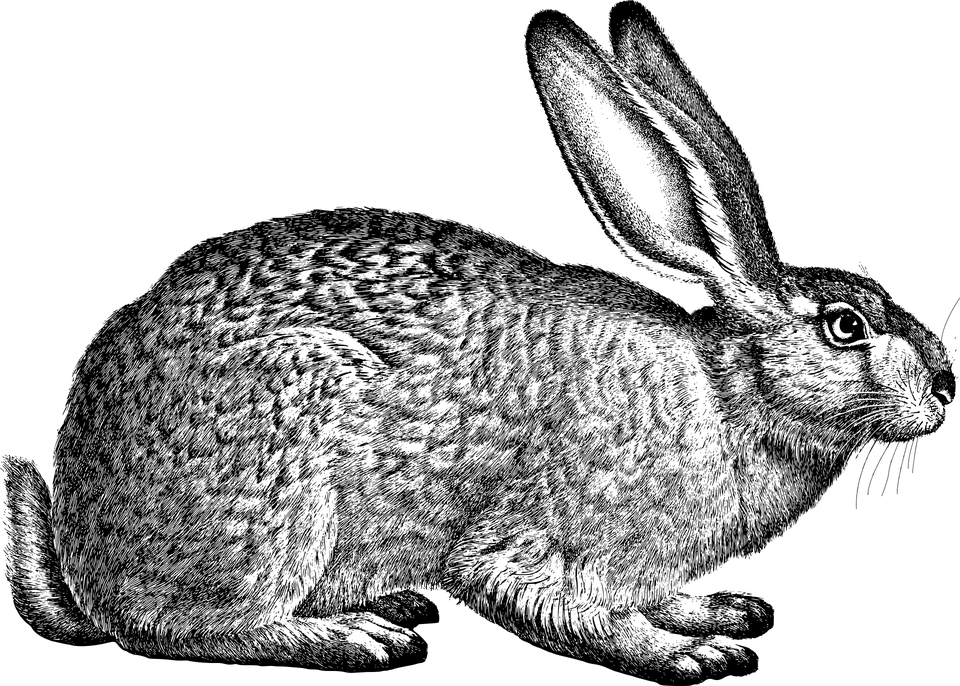
\includegraphics[width=4in,height=\textheight]{./rabbit.png}

Welcome to experimental design. There are two sets of three exercises provided to explore principles for better experiments. This is a simple book to support the practical, at-home learning associated with experimental design. The text `Experimental Design for the Life Sciences' underpins the design principles \citep{RN6381}.

There are two primary modules.

\begin{enumerate}
\def\labelenumi{(\arabic{enumi})}
\item
  Field experiments comprises three outdoor experiments to explore sampling heterogeneous, complex processes in natural systems. The purpose is to provide choice. You need to try each, briefly, as a pilot experiment only. Then, select one to pursue in depth and write up as a research article.
\item
  The data experiments describe the opportunity to use design thinking to structure existing data that others have already collected. The same principles for better experiments still apply in how you reuse the data. There are also three examples provided. Select only one and write up as a note.
\end{enumerate}

Both report formats supported by \href{https://www.facetsjournal.com/about/}{FACETS}. It is the first and only open access science journal in Canada.

\hypertarget{field-experiments-gear-and-prep}{%
\subsubsection*{Field experiments gear and prep}\label{field-experiments-gear-and-prep}}
\addcontentsline{toc}{subsubsection}{Field experiments gear and prep}

\hypertarget{data-design-experiment-prerequisites}{%
\subsubsection*{Data-design experiment prerequisites}\label{data-design-experiment-prerequisites}}
\addcontentsline{toc}{subsubsection}{Data-design experiment prerequisites}

\hypertarget{birds}{%
\chapter{Balcony birdwatching}\label{birds}}


\includegraphics[width=4in,height=\textheight]{./owl.png}\\
Bird observation, from a distance.

\hypertarget{steps}{%
\subsubsection*{Steps}\label{steps}}
\addcontentsline{toc}{subsubsection}{Steps}

\begin{enumerate}
\def\labelenumi{\arabic{enumi}.}
\tightlist
\item
  Scout out a location with more than a single species of birds and a frequency of a few different individuals of birds over a 5-10 minute duration.\\
\item
  Select a good spot to the observe birds at your designated location. It can be a balcony or quiet spot. Vegetation such as trees or shrubs can facilitate observation of birds by providing habitat.\\
\item
  Choose a distance that permits enough resolution to see plumage and what an individual bird is doing (depending on whether you are using binoculars, a spotting scope, or unassisted with your vision). There are considerable merits to observing birds more simply \citep{RN6773}. You are also welcome to address any visibility or spotting challenges using bird calls to record frequency of birds in a sampling region.\\
\item
  Specify a duration to sample, for instance, 60 minutes when you have observed the most birds in your scouting exercise. Remember, this is a pilot experiment. Take qualitative notes, sketch, and complete this datasheet.\\
\item
  Use your notes to complete a meta-data file, i.e.~a description of how the data were collected, whether, when, and what each attribute in your dataset means.\\
\item
  Sign out a bird guide for your region from the library or university or try out a \href{https://www.birds.cornell.edu/k12/best-apps-for-birding-with-kids/}{free app} for now to support identification.
\end{enumerate}

\hypertarget{data}{%
\subsubsection*{Data}\label{data}}
\addcontentsline{toc}{subsubsection}{Data}

\href{./birds.csv}{Here} is a sample datasheet for the pilot experiment. This is set up as species-level observations, i.e.~each row or replicate is a species of bird you observe. This datasheet is for the pilot experiment, and it is a stepping stone for the deeper dive experiment if you choose to complete this experiment for your first report. A more detailed datasheet can consider duration or start and stop times of each individual bird, more details on the environment, or record interesting ecological or environmental variables that are present in the environment too - noise, disturbance, squirrels, other birds, etc.

\hypertarget{meta-data}{%
\subsubsection*{Meta-data}\label{meta-data}}
\addcontentsline{toc}{subsubsection}{Meta-data}

In many disciplines of science, meta-data are the descriptive elements of the dataset. They provide a clear means for discovery and reuse of data collected - by you in future and for others \citep{RN3201, RN6774}. For the purposes of our practical learning in experimental design here, describe what each column in our dataset means, describe the structure of your dataset (i.e.~each row is a species-level observation, or plot, or transect), describe the duration of sampling, location, and provide a bit of guidance for someone to use in inspecting the dataset. It is very similar to the methods in conventional publications or standard reports, but it ensures each attribute in the dataset has a brief description. It is also superb preparation for the methods if you choose to write a report.

\hypertarget{deeper-dive}{%
\subsubsection*{Deeper dive}\label{deeper-dive}}
\addcontentsline{toc}{subsubsection}{Deeper dive}

If you choose this adventure, your goal is to experiment with the method of animal observation to test a hypothesis and predictions. The text `Experimental Design for the Life Sciences' does an excellent job of explaining how to set up hypotheses and predictions \citep{RN6381}. Pilot experiment first, think, explore your data and notes, then write your ideas down that you want to test. A hypothesis is a clear explanation of how a system works \citep{RN6776, RN6775}. The predictions are logical and resonable outcomes if the hypothesis is a good approximation of how the system works, i.e.~the key variables that make it work. Predictions should be testable and read like simple sentences that describe results. The goal of the deeper-dive experiment is to take your pilot experiment, examine what worked and did not work so well in your experiment, and do a deeper and more thorough job of testing a key idea that you are interested in associated with bird communities in your backyward or neighbourhood. The goal should be to explore one key factor the describes how the species locally interact within one another, the environment or other species, or resources.

\hypertarget{bioblitz}{%
\chapter{Backyard bioblitz}\label{bioblitz}}

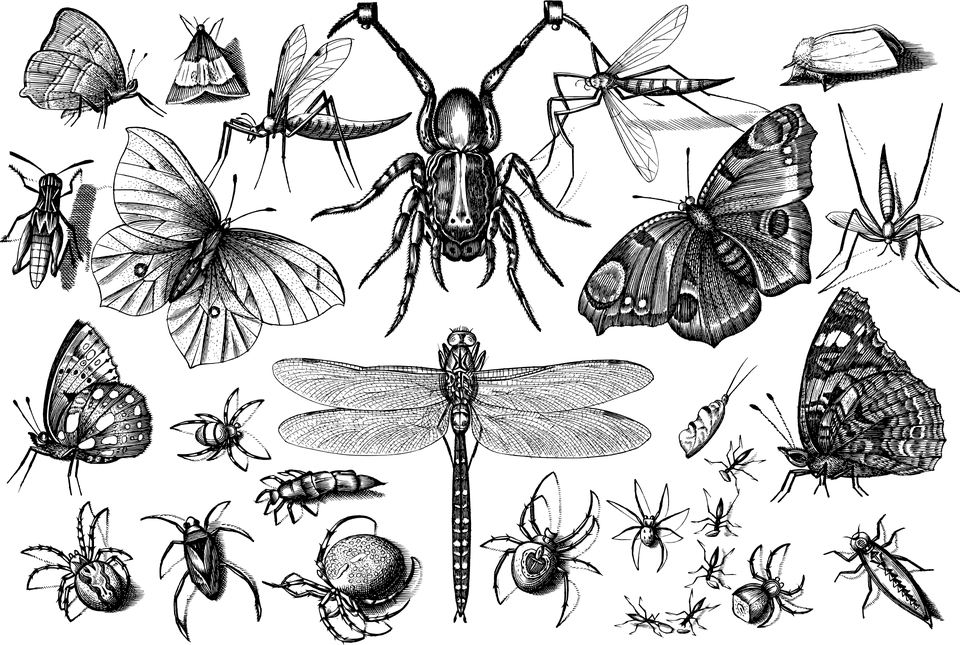
\includegraphics[width=4in,height=\textheight]{./insects.png}

A bioblitz is a biodiversity survey that is done rapidly for a specific place.

\hypertarget{survey}{%
\chapter{Solo surveys}\label{survey}}

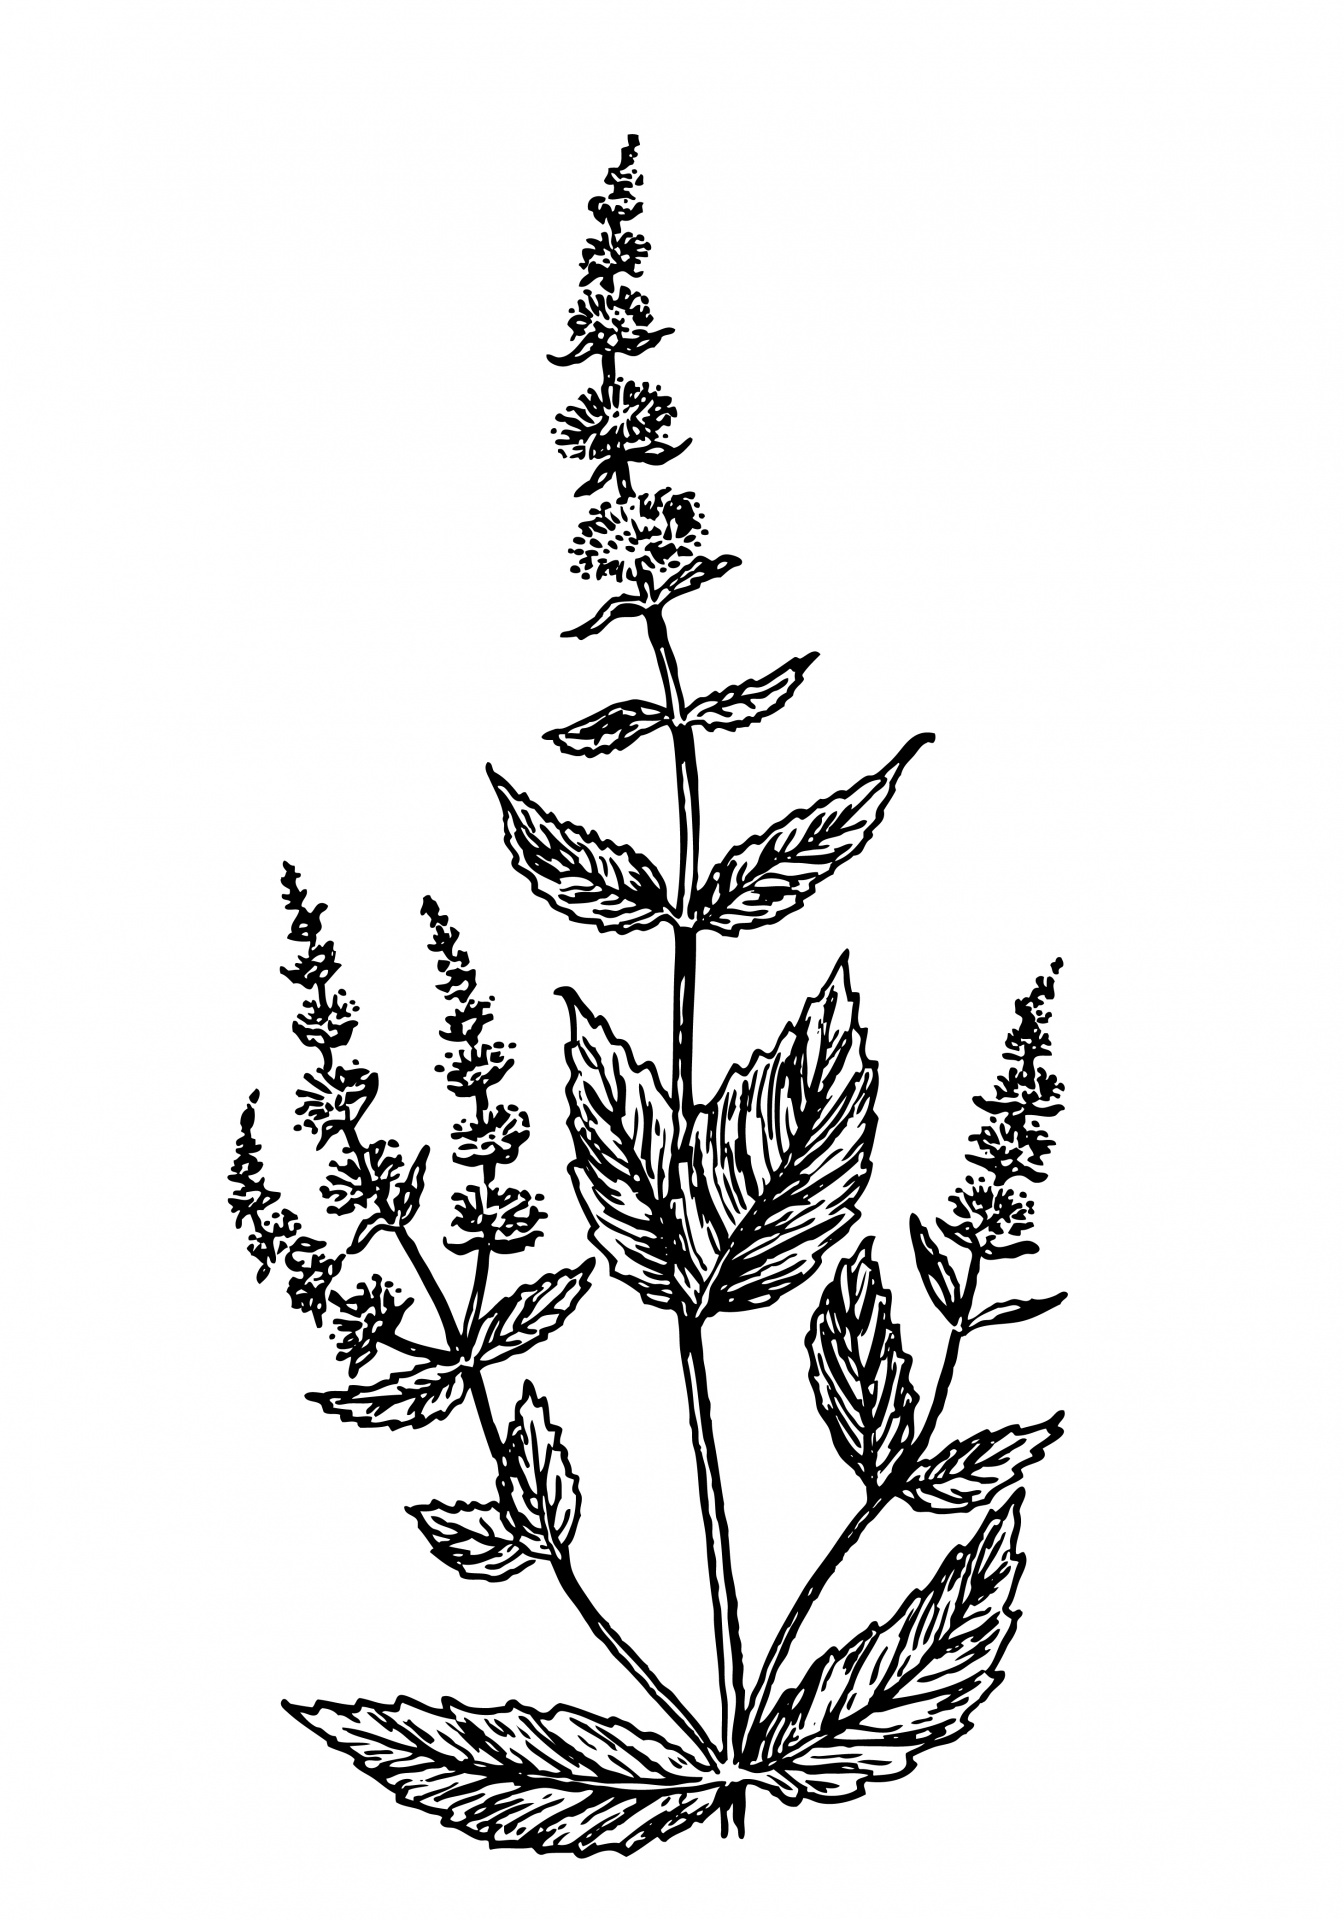
\includegraphics[width=4in,height=\textheight]{./plant.jpg}

Distributed ecological networks often use surveys done by individuals or small-teams to compile data on species or communities. Transects and quadrats are typically used to structure these `walk-through' surveys to estimate abundances and distributions of focal species.

\hypertarget{magic}{%
\chapter{Magic data}\label{magic}}

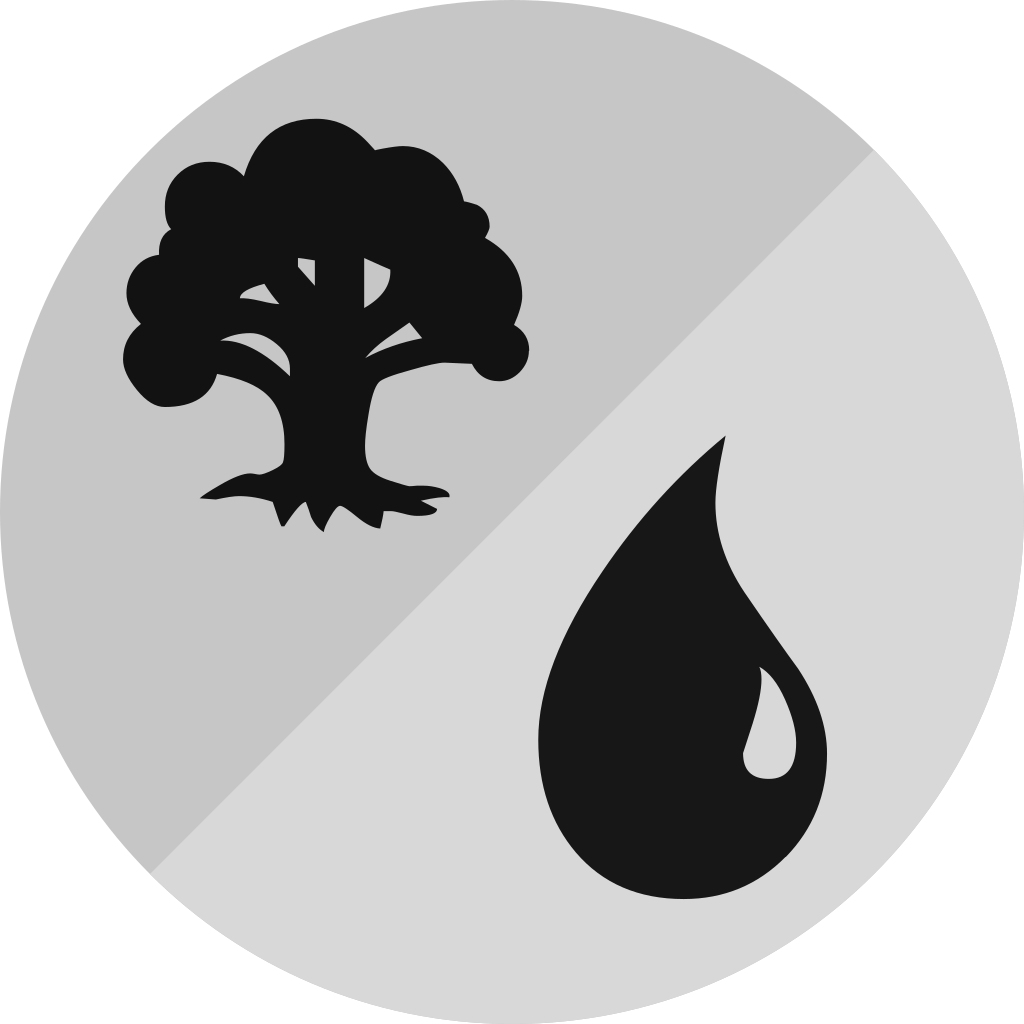
\includegraphics[width=4in,height=\textheight]{./magic.png}

Magic the Gathering is a popular collectible card game that includes strategy and chance.

\hypertarget{diversity}{%
\chapter{Diversity data}\label{diversity}}

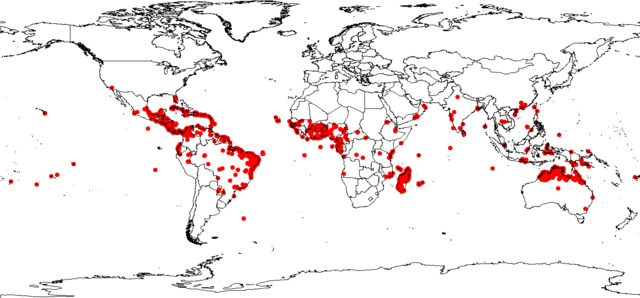
\includegraphics[width=4in,height=\textheight]{./gbif.png}

Diversity data from ebird or any citizen science project.

\hypertarget{humans}{%
\chapter{Human data}\label{humans}}

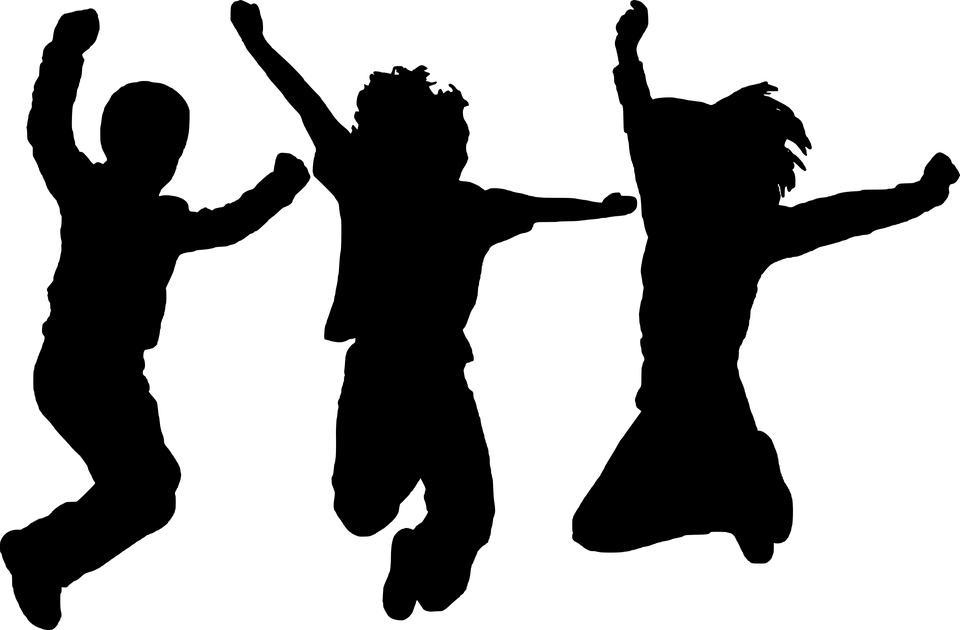
\includegraphics[width=4in,height=\textheight]{./humans.png}

Data associated with humans. Fitbit steps and sleep.

\hypertarget{notes}{%
\chapter{Final notes}\label{notes}}

Observations and conclusions.

  \bibliography{book.bib,packages.bib}

\end{document}
